%!TEX root = ../../thesis.tex

\section{RV precision update}
\label{}
As detailed in the \cref{sec:eniric} updating the software introduced several changes that affect the {RV} precisions values slightly, the numerical gradient, and the masking order for Condition~\#2 and more importantly the bug also found with Condition~\#2.

The 180 spectral combinations from \citet{figueira_radial_2016}, are repeated here using \eniric{} to have an updated and corrected table of relative {RV} precisions.
This table is given in \cref{tab:rv_aces_btsettl}, calculated using the {PHOENIX-ACES} spectra and also the {BT-Settl} models.
 
The precision changes are visually represented in \cref{fig:figueria_comparision} by comparing Figure~1 of \citet{figueira_radial_2016} (left) to an updated version(right).
Each panel shows the precision achieved as a function of spectral band for stars with a rotational velocity of \Vsini=1.0\kmps{} and spectral types M0 (3900\K), M3 (3500\K), M6 (2800\K), and M9 (2600\K).
The dashed line represents the theoretical limits imposed by Condition \#1, and the filled area represents the values within the limits set by Conditions~\#2 (circles) and \#3 (triangles); blue, green, and red represent the results obtained for resolutions of 60000, 80000, and 100000, respectively.
The spectra were normalized to have a \snr{} of 100 per resolution element as measured at the centre of the \emph{J}-band.

The values for Condition~\#1 and \#3 only have small differences which is barely noticeable, while Condition~\#2 has large band dependant changes, shown by the change in the shaded areas.
For example the that \emph{Z} and \emph{J}-band RV precisions decrease with the new results, while the {K} band gets substantially worse.
This occurs because the software did not mask many of the regions affected by telluric lines, where as in the new results, a significant portion is masked out due to the overlap of telluric lines, leading to a higher \(\delta V_{\rms}\) value.
The \emph{H}-band also sees a small increase in \(\delta V_{\rms}\).
As stated previously the discovery of the bug affecting telluric masking does not change the conclusions of \citet{figueira_radial_2016}.

These updated {PHOENIX-ACES} values will be published in an upcoming work as an amendment to the \citep{figueira_radial_2016} values.

\begin{figure}
    \centering
    \begin{tabular}{cc}
        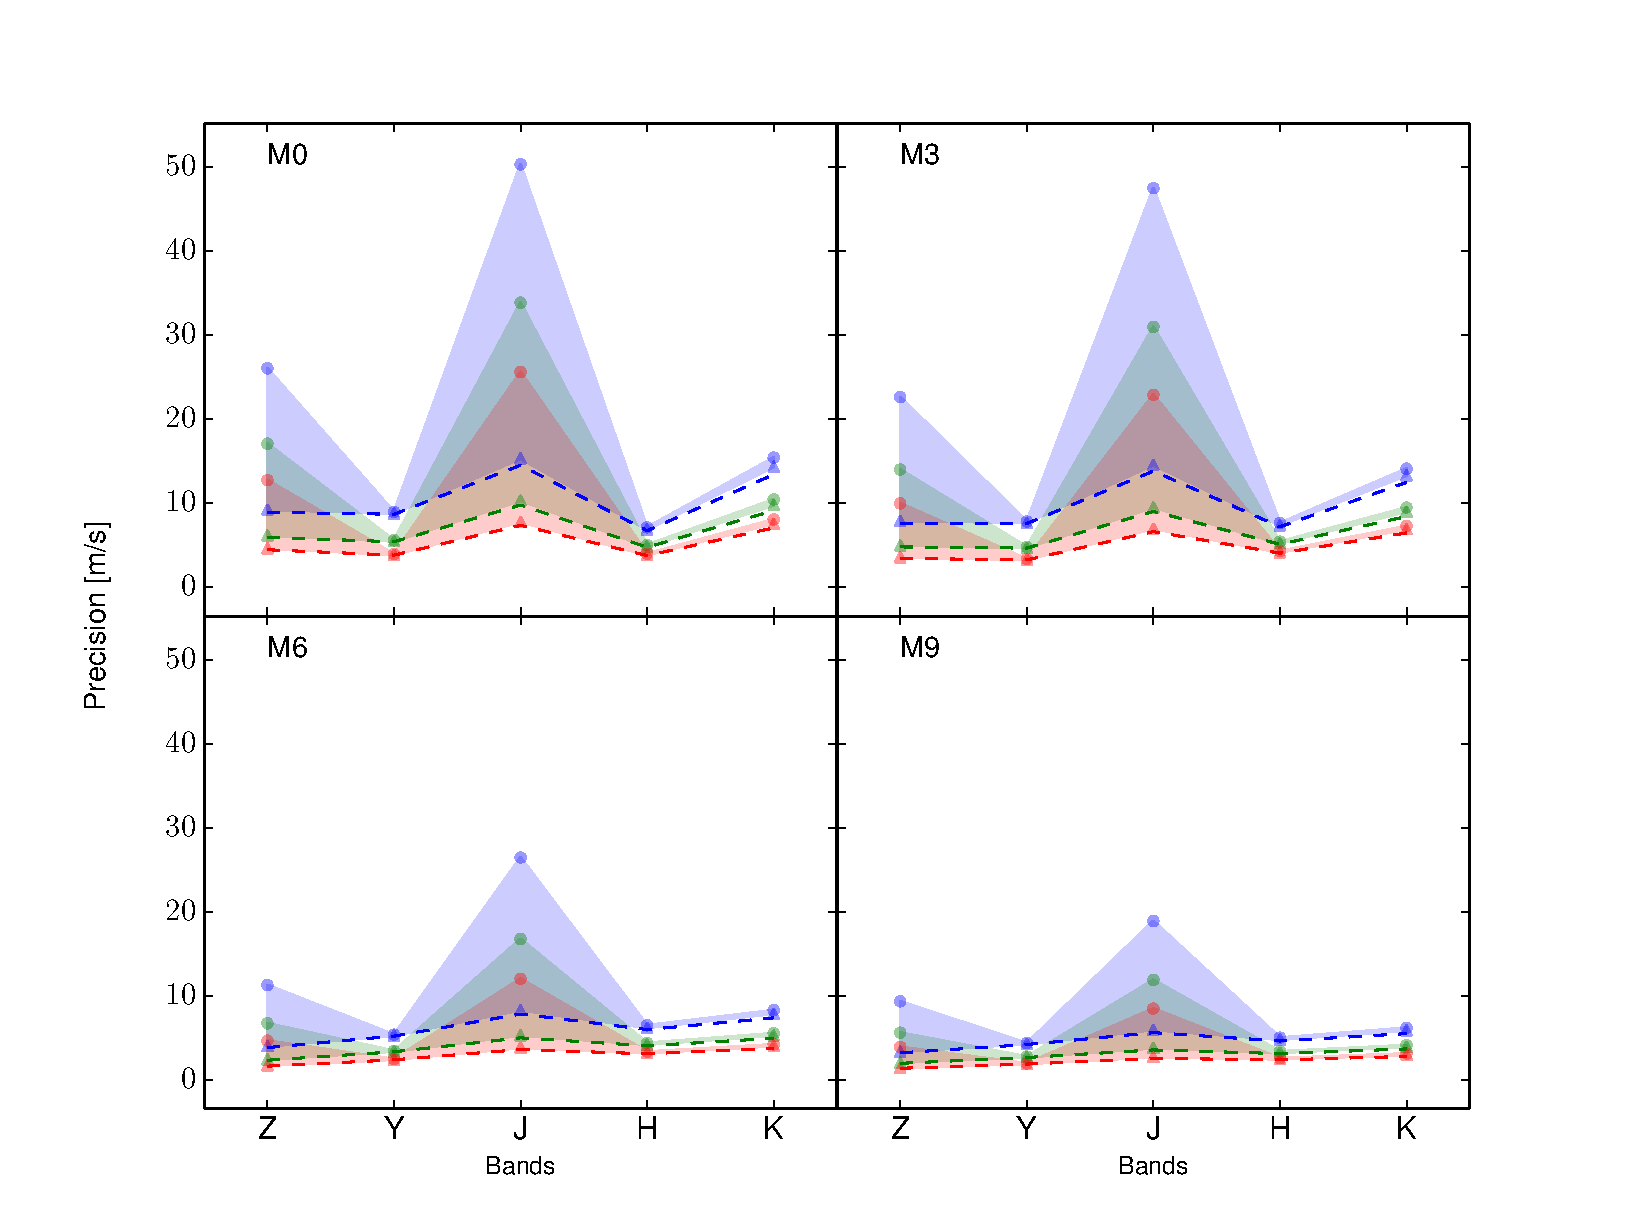
\includegraphics[width=0.48\linewidth]{figures/information-content/Rvprec_vsini1.pdf} &  % Figueria plot
        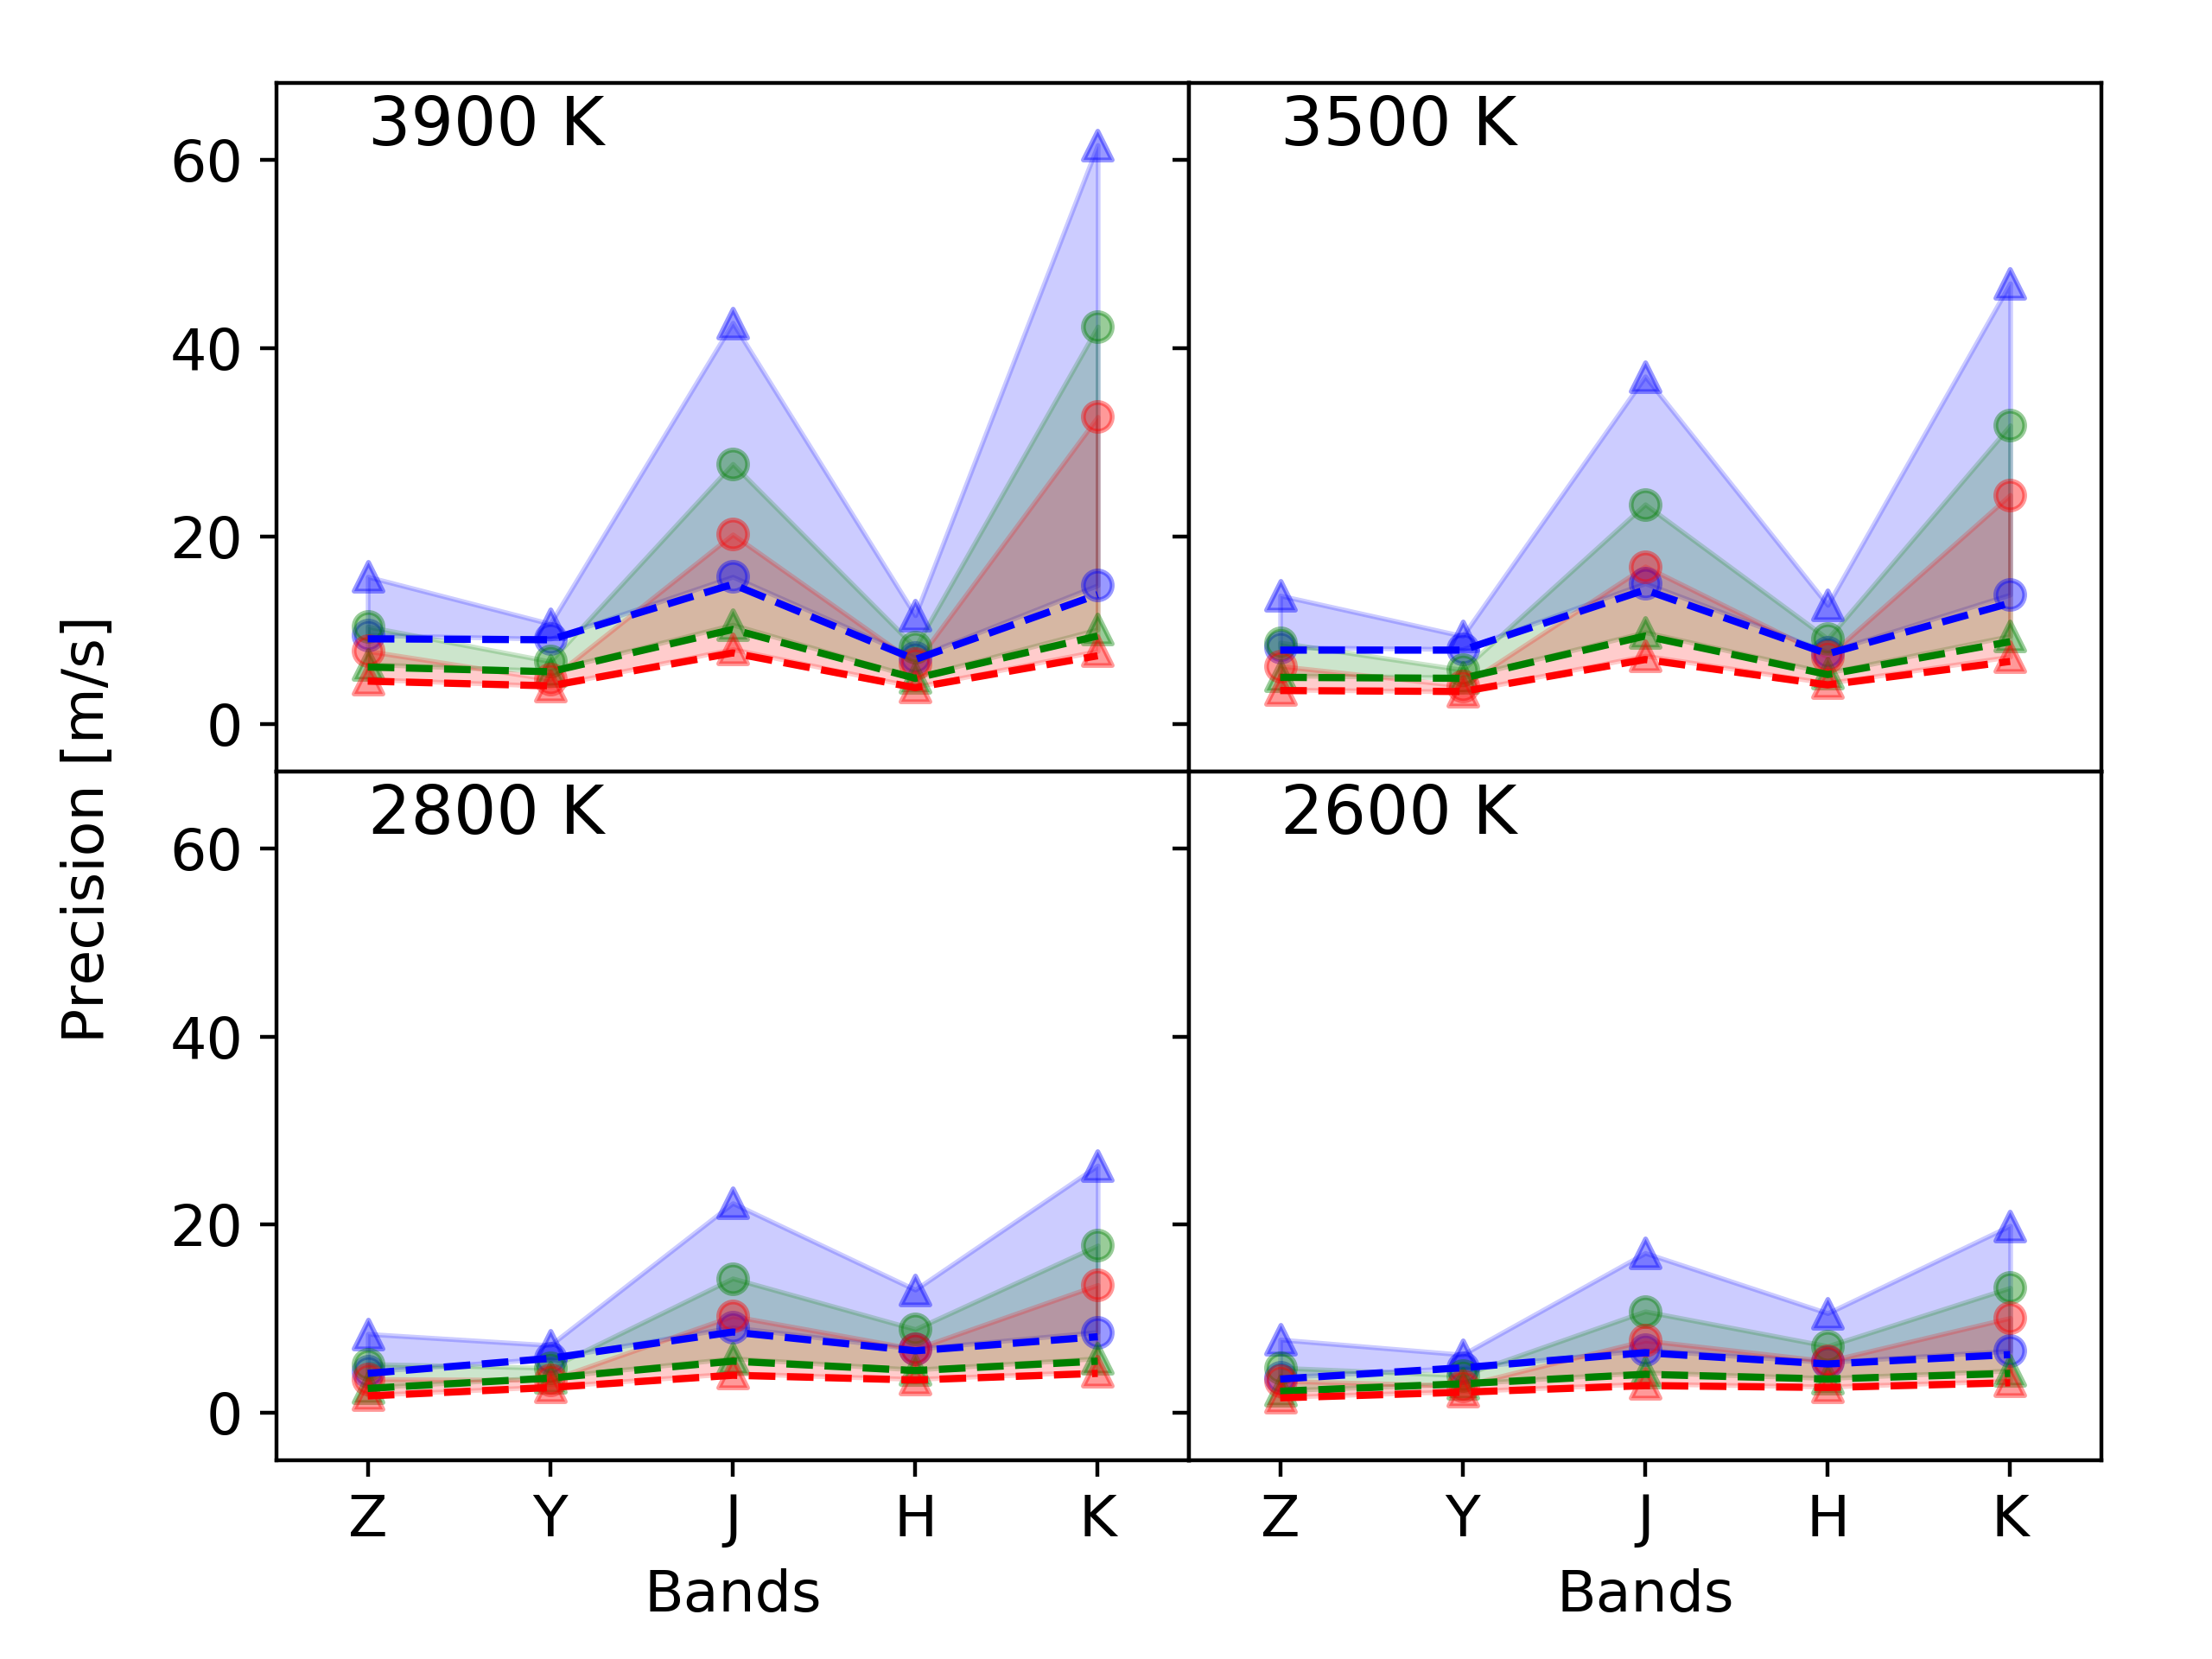
\includegraphics[width=0.47\linewidth]{figures/information-content/precision_fourpanel.png}\\ % eniric plot
    \end{tabular}
    \caption[Comparision of {RV} precision results to~\citet{figueira_radial_2016}.]{Comparison of the updated precision values.
        Each panel shows the precision achieved as a function of spectral band for stars with a rotational velocity of \Vsini=1.0\kmps{} and spectral types M0 (3900\K), M3 (3500\K), M6 (2800\K), and M9 (2600\K).
        The dashed line represents the theoretical limits imposed by Condition \#1, and the filled area represents the values within the limits set by Conditions~\#2 (circles) and \#3 (triangles); blue, green, and red represent the results obtained for resolutions of 60\,000, 80\,000, and 100\,000, respectively.
        The spectra were normalized to have a \snr{} of 100 per resolution element as measured at the centre of the \emph{J}-band.
        Left: Figure~1 from~\citet{figueira_radial_2016}.
        Right: Updated precision values computed using \eniric{}.
        The main difference is the area of shaded region due to the problem identified with Condition~\#2 (which is the upper edge).}
    \label{fig:figueria_comparision}
\end{figure}
\todo{Change to 55\mps{} upper limit?}



\begin{figure}
    \centering
    \begin{tabular}{cc}
    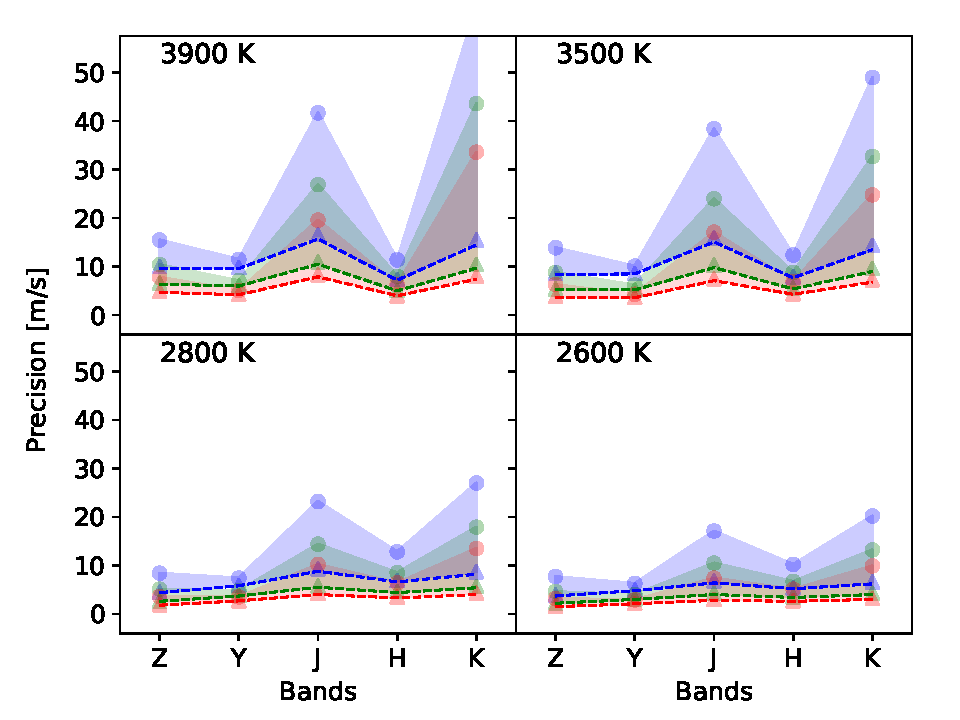
\includegraphics[width=0.47\linewidth]{figures/information-content/aces_4panel} &
    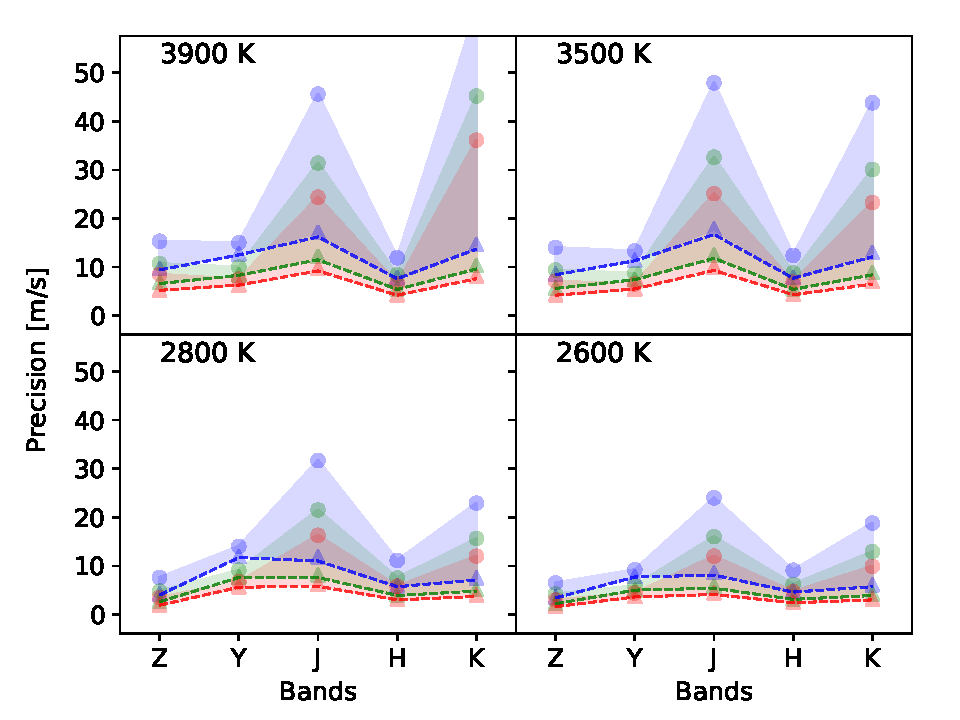
\includegraphics[width=0.47\linewidth]{figures/information-content/btsettl_4panel}\\
    \end{tabluar}
    \caption{ACES and BT-Settl models}
    \label{fig:precision_aces_btsettl}
\end{figure}

In comparing the BT-Settl values ....

\todo{side by side with BT-settl} 


\section{Metallicity and \Logg{}}
\label{sec:metallicity_logg}

\begin{figure}
    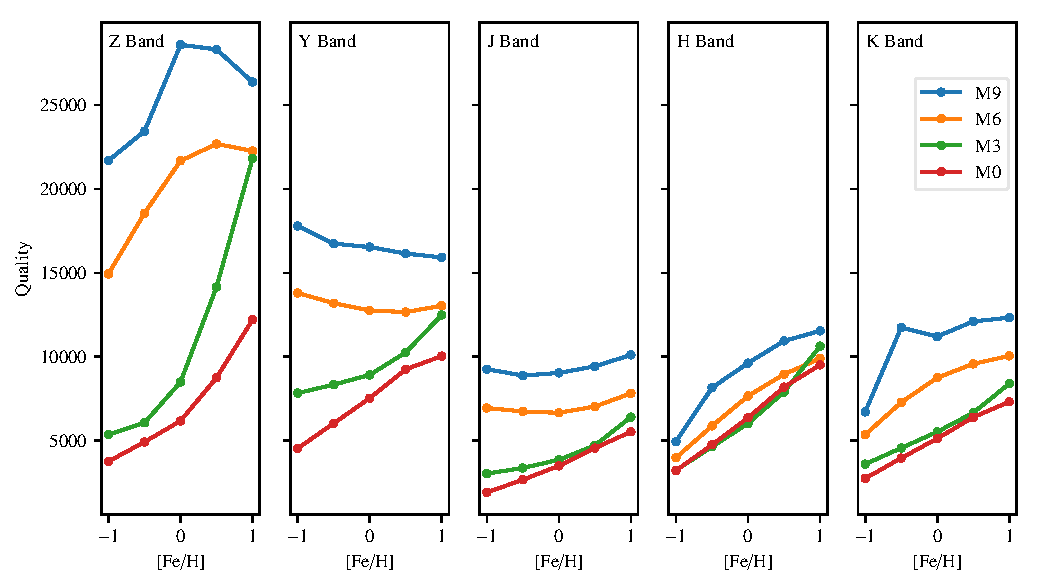
\includegraphics[width=0.99\linewidth]{figures/information-content/metalicity_effect.pdf}\\
    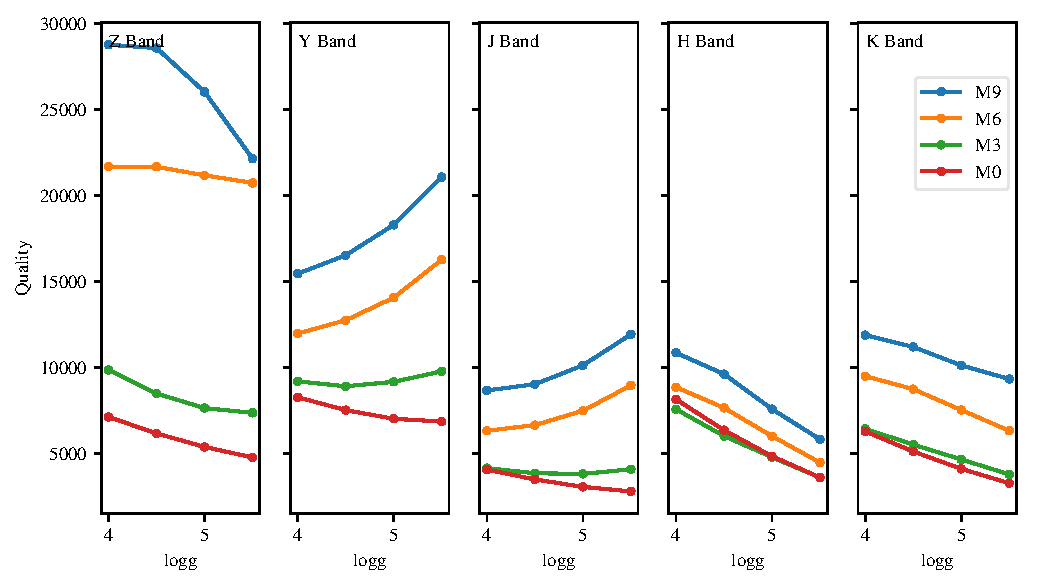
\includegraphics[width=0.99\linewidth]{figures/information-content/logg_effect.pdf}
    \caption[Quality factor verse \feh{} and \Logg{} for different spectral types and wavelength bands.]{Quality factor changes across spectral type and bands for variations in \feh{} and \Logg{}.
        Broadening values are R=100\,000 and \Vsini{}=1.0\kmps{}.
        Top: Quality factor variation of \feh{} between -1.0 to 1.0 at a fixed \Logg{}=4.5.
        Bottom: Quality factor variation of \Logg{} between 4 and 5.5 with fixed \feh{}=0.0.
        Note a higher quality factor corresponds to an increased {RV} precision.}
    \label{fig:deviations}
\end{figure}

With the ability to explore a wider range of parameters the range of {PHOENIX-ACES} models extended to explore the \Logg{} and metallicity of the {PHOENIX-ACES} models.
\Eniric{} was to compute the spectral quality factor, \(Q\) (\cref{eqn:quality_factor}), and {RV} precision for all {PHOENIX-ACES} models with \Logg{} between 4.0--5.5 and \feh{} between -1--1, inclusive.
The spectral factor is used for the comparison following, \citet{artigau_optical_2018} in which it was used to compare between models, and observed spectra, independent of the flux levels.
Since \(Q\) is inversely proportional to \(\delta V_{\rms}\) a higher \(Q\) is better.

The spectral quality factor variations for the {M-dwarf}s M0, M3, M6, M9, with a broadening of R=100\,000 and $\vsini=1.0$\kmps{} across the \nir{} bands is shown \cref{fig:deviations}. The top row shows the Quality factors for model spectra with a fixed \Logg=4.5 but the have a variable \feh{} between -1.0 to 1.0.
The bottom row shows the opposite, a fixed \feh{}=0.0 while the \Logg{} is varied between 4 and 5.5.
The five separate plots in each row represent the \nir{} wavelength bands \emph{Z}--\emph{K} and the four different coloured line are the different M-dwarfs (blue M9, orange M6, green M3, red M0).
Note the cooler M-dwarfs have higher spectral quality factors.
\todo{}

Multiple effects are observed in this figure which are identified below.


The \emph{Z}-band has a large separation in spectral quality due to spectral type, this is because the continuum the \emph{Z}-band is severely eroded in the spectra of late M's as they cool.
Each spectral type also behaves very differently to a change in \feh{} and \Logg{}.
For {M0} and {M3} there is an increase with \feh{} below solar metallicity, above solar metallicity the slopes of the lines dramatically increase, especially for {M3}.
For {M6} and {M9} there is a step slope with \feh{} below solar metallicity, which flattens off at solar metallicity, and even decreases for the {M9} spectra above solar metallicity.
As \Logg{} increases in the \emph{Z}-band there is a decrease in quality.
There is a consistently large separation between early and late M's that.
The quality for {M6} is very shallow, while for {M9} the quality is nearly flat for \Logg{}=4.0 and 4.5 but then decreases sharply at higher \Logg{}.

\emph{Y}-band -\\

\emph{J}-band - \\

For the H and \emph{K}-band there is fairly consistent linear trend for all spectral types, with the quality factor increasing with an increase in \feh{} and decreasing with an increase in \Logg{}.
There is also only a relatively small variation in quality factor due to the spectral type.



\clearpage


\section{{SPIRou} and {NIRPS} {ETC}}\label{sec:spirou_nirps_etc}
Having this tool to calculate {RV} precisions efficiently lead to contributions to the Exposure Time Calculators (ETC) for both the {SPIRou} and {NIRPS} spectrographs. Both of these were at the request of the respective instruments.

In September 2017 \eniric{} was used to provide precision calculations for the {SPIRou} ETC\footnote{\url{http://www.cfht.hawaii.edu/Instruments/SPIRou/SPIRou_etc.php}}.
These were the same spectral parameters as~\citet{figueira_radial_2016} except with the precisions for each band referenced to {\snr{}=100} in its own band.
The modification of \cref{subsec:snr_scaling} was made to fulfil this request. These values are given in \cref{tab:spirou_precisions}.

In May 2018 \eniric{} was used provide precision calculations for the {NIRPS} {ETC}.
This extended the spectral range from {M0}, {M3}, {M6}, {M9} at 3900, 3500, 2800, 2600\K{} respectively, but to all temperatures between 2500\K{} and 4000\K{} inclusively.
This provides a finer resolution coverage over the M spectral type, allowed by the {PHOENIX-ACES} library.
Instrumental resolutions of 75\,000 and 100\,000 were requested to match the {NIRPS} instrument.
The \Logg{} and metallicity, sampling rate remained at the~\citet{figueira_radial_2016} levels of 4.5, \textbf{0.0} and 3.0 respectively.
Precisions were provided for \snr{} of 100 relative to the \emph{J}- and \emph{H}-bands as well as to each band individually.
Artigua (\emph{priv. comm.} 2018) suggested the truly relevant values would be the \snr{} in \emph{H}-band for {NIRPS} instrument.
The values calculated for {NIRPS} are given in \cref{tab:nirps_precisions}.

The result tables, along with the command line incantation are detailed in \cref{app:nir_prec_amendment}.




